
    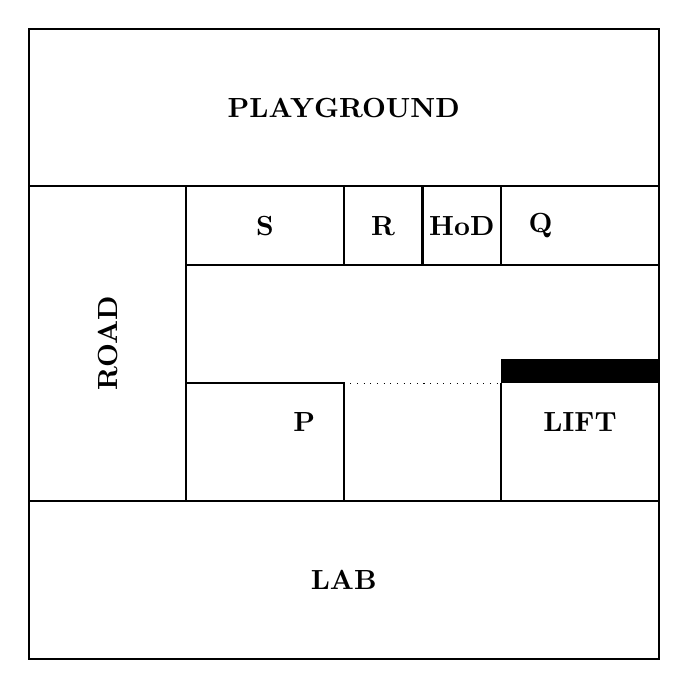
\begin{tikzpicture}
        % Outer boundary
        \draw[thick] (0,0) rectangle (8,8);
        
        % Divisions
        \draw[thick] (0,6) -- (8,6); % Horizontal line for playground
        \draw[thick] (0,2) -- (8,2); % Horizontal line for lab
        \draw[thick] (2,6) -- (2,2); % Vertical line for road
        \draw[thick] (6,3.5) -- (6,2); % Vertical line for lift
\draw[thick](2,5)--(8,5);
        % Playground and Lab Labels
        \node at (4,7) {\textbf{PLAYGROUND}};
        \node at (4,1) {\textbf{LAB}};

        % Road label
        \node[rotate=90] at (1,4) {\textbf{ROAD}};
        
        % Lift Label
        \node at (7,3) {\textbf{LIFT}};

        % HoD, Q, R, S labels
        \draw[thick] (2,6) -- (2,5); % Horizontal line for HoD row
        \draw[thick] (4,6) -- (4,5); % Vertical line for Q
        \draw[thick] (5,6) -- (5,5); % Vertical line for R
        \draw[thick] (6,6) -- (6,5); % Vertical line for S
        
        \node at (3,5.5) {\textbf{S}};
        \node at (4.5,5.5) {\textbf{R}};
        \node at (5.5,5.5) {\textbf{HoD}};
        \node at (6.5,5.5) {\textbf{Q}};

        % P label
        \draw[thick] (2,3.5) -- (4,3.5)--(4,2); % Horizontal line for P row
        \draw[dotted](4,3.5)--(6,3.5);
        \node at (3.5,3) {\textbf{P}};
        
        % Lift black bar
        \fill[black] (6,3.5) rectangle (8,3.8); % Thick black bar for the lift

    \end{tikzpicture}
